\documentclass[dvipdfmx]{jsarticle}
\usepackage[dvipdfmx]{hyperref, xcolor, graphicx}
\hypersetup{
    colorlinks=true,
    citecolor=blue,
    linkcolor=blue,
    urlcolor=blue,
}

% 数式
\usepackage{amsmath,amsfonts,amssymb,amsthm, mathtools}
\usepackage{bm}
\usepackage{physics}
\usepackage{tcolorbox}
\tcbuselibrary{breakable} % 必要に応じて

\newtcolorbox{mybox}[1][]{%
  title=#1,
  fonttitle=\gtfamily\sffamily\bfseries,
  colframe=blue,
  colback=blue!3!,
  breakable, % 長文対応したい場合
}

\usepackage[dvipdfmx]{graphicx}
\usepackage{tikz} %図を描く
\usetikzlibrary{positioning, intersections, calc, arrows.meta,math} 

\usepackage{here}

\begin{document}

\section{Bayes理論の目的}
Bayes理論は、パラメータの集合$W \subset \mathbb{R}^d$、真の分布$q(x)$、確率モデル$p(x|w)$、事前分布$\varphi(w)$が事前に与えられて構築される理論である。
理論の目的は以下のようにまとめられる:
\begin{mybox}[Bayes理論の目的]
    真の分布$q(x)$、確率モデル$p(x|w)$、事前分布$\varphi(w)$が与えられたとする。
    自然数$n=1,2,3,\ldots$に対して、我々は何らかの処方箋に従って予測分布と呼ばれる確率分布の系列$\{p_n^{*}(x)\}_{n=1}^{\infty}$を構成する。
    予測分布の構成手法はBayes推測、事後確率最大化法、最尤推定法、平均プラグイン法などが存在する。
    たとえばBayes推測を用いた場合では、予測分布を
    \begin{equation}
        p_{n}^{*}(x) \coloneqq \int p(x|w)p(w|X^n)\,\dd{w} = \ev{p(x|w)}_{w|X^n}
    \end{equation}
    と定める。
    ここで、$p(w|X^n)$は事後分布と呼ばれる確率分布であり、真の分布$q(x)$から得られる$n$個の独立なサンプル$X^n$(データセット)を用いて、
    \begin{equation}
        p(w|X^n) \propto \varphi(w)\prod_{i=1}^{n}p(X_i|w)^{\beta}
    \end{equation}
    と定義される。Bayes理論の主な目的は、予測分布の構成手法としてBayes推測を用いた場合、$n$の増大に対して
    \begin{equation}
        D_{\text{KL}}[q(x) \parallel p_n^{*}(x)] = \int q(x)\ln\frac{q(x)}{p_n^{*}(x)}\,\dd{x} = \mathbb{E}_X\qty[\ln\frac{q(x)}{p_n^{*}(x)}]
    \end{equation}
    がどのような振る舞いをするか、すなわちどのように予測分布$p_n^*(x)$が真の分布$q(x)$に近づいていくかを調べることが目的である。
    また、
    \begin{equation}
        D_{\text{KL}}[q(x) \parallel p_n^{*}(x)] = \mathbb{E}_X[\ln{q(x)}] - \mathbb{E}_X[\ln{p_n^{*}(x)}]
    \end{equation}
    であり、右辺第一項は真の分布のみで定まる定数である。したがって右辺第二項の振る舞いを調べられれば良い。
    予測分布をBayes推測で構成した場合、
    \begin{equation}
        - \mathbb{E}_X\qty[\ln{p_n^{*}(x)}] = -\mathbb{E}_X\qty[\ln\ev{p(X|w)}_{w|X^n}]
    \end{equation}
    となり、この値は汎化損失$G_n$と呼ばれるものになっている:
    \begin{equation}
        G_n \coloneqq -\mathbb{E}_X\qty[\ln\ev{p(X|w)}_{w|X^n}]\;。
        \label{eq:bayes-goal}
    \end{equation}
    しかし我々は真の分布にアクセスできないため、原理的に$G_n$の値を求めることはできない。
    Bayes理論の目的を言い換えると、この$G_n$の値をいかにして推定するかということになる\footnote{
        原理的に計算可能な$T_n$を推定量として見るのではだめ?$G_n$を推定すること自体をしたいわけではない?
        たぶん情報量規準はこの疑問と関係している気がする。
    }。特に
    \begin{itemize}
        \item 事後分布による期待値計算を如何にして実行するか(原理的には計算可能だが…?)
        \item 真の分布による期待値計算をどのような推定量として評価するか
    \end{itemize}
    ということが重要である。また、$G_n$は出現サンプルに依存した値であることにも注意。
\end{mybox}
\newpage
事後分布はモデルと事前分布から定まるため、原理的には計算可能である。実用上では、事後分布やモデルが複雑であれば積分計算が実行できないため、
積分の収束先からのズレを見るオーダー評価しか行えない。オーダー評価の処方箋を与えているのが正則理論や一般理論と呼ばれる理論である。

{\color{red}{(情報量規準についてまだ理解してないので、この段落は自分の予想)}}真の分布による期待値計算は、原理的に何らかの推定量として扱う必要がある。
推定量として扱う方法を与えるために、情報量規準と呼ばれる量を導入する。
そのため、異なる情報量規準を用いると異なる推定結果となり、評価の意味合いが変わってくる。

\subsection{いくつかの概念の定義と本書の仮定について}

\begin{mybox}[真の分布に対して最適なパラメータの集合]
    パラメータの集合$W$に対し、真の分布$q(x)$とモデル$p(x|w)$の間のKL divergenceを最小にするパラメータの集合を$W_0$と定義する:
    \begin{equation}
        W_0 \coloneqq \{ w \in W \mid w = \arg\min_{w} D_{\mathrm{KL}}[q(x) \parallel p(x|w)] \}
        \label{eq:optimal-parameter-set}
    \end{equation}
    この集合のことを、真の分布に対して最適なパラメータの集合と呼ぶ。
\end{mybox}

\begin{mybox}[実質的にユニーク]
    任意の$w_0\in W_0$について、$p(x|w_0)$がユニークな確率分布$p_0(x)$を表すとき、真の分布に対して最適な確率分布は実質的にユニークであるという。
\end{mybox}
以下では実質的にユニークが常に実現されていることを仮定する。
渡辺ベイズ本では、より強い仮定として、「相対的に有限な分散を持つ」という状況が達成されていることを仮定する。
\footnote{「相対的に有限な分散を持つ」ことが達成されていない場合、後で定義する重要な量である$K_n(w)$の分散がその平均でバウンドできなくなるため、
事後分布がサンプルに応じて大きく変動してしまうことが問題となるらしいです。これ以上はよくわからないです。(渡辺ベイズ p36, 注意12を参照。)}

\begin{figure}[H]
    \centering
    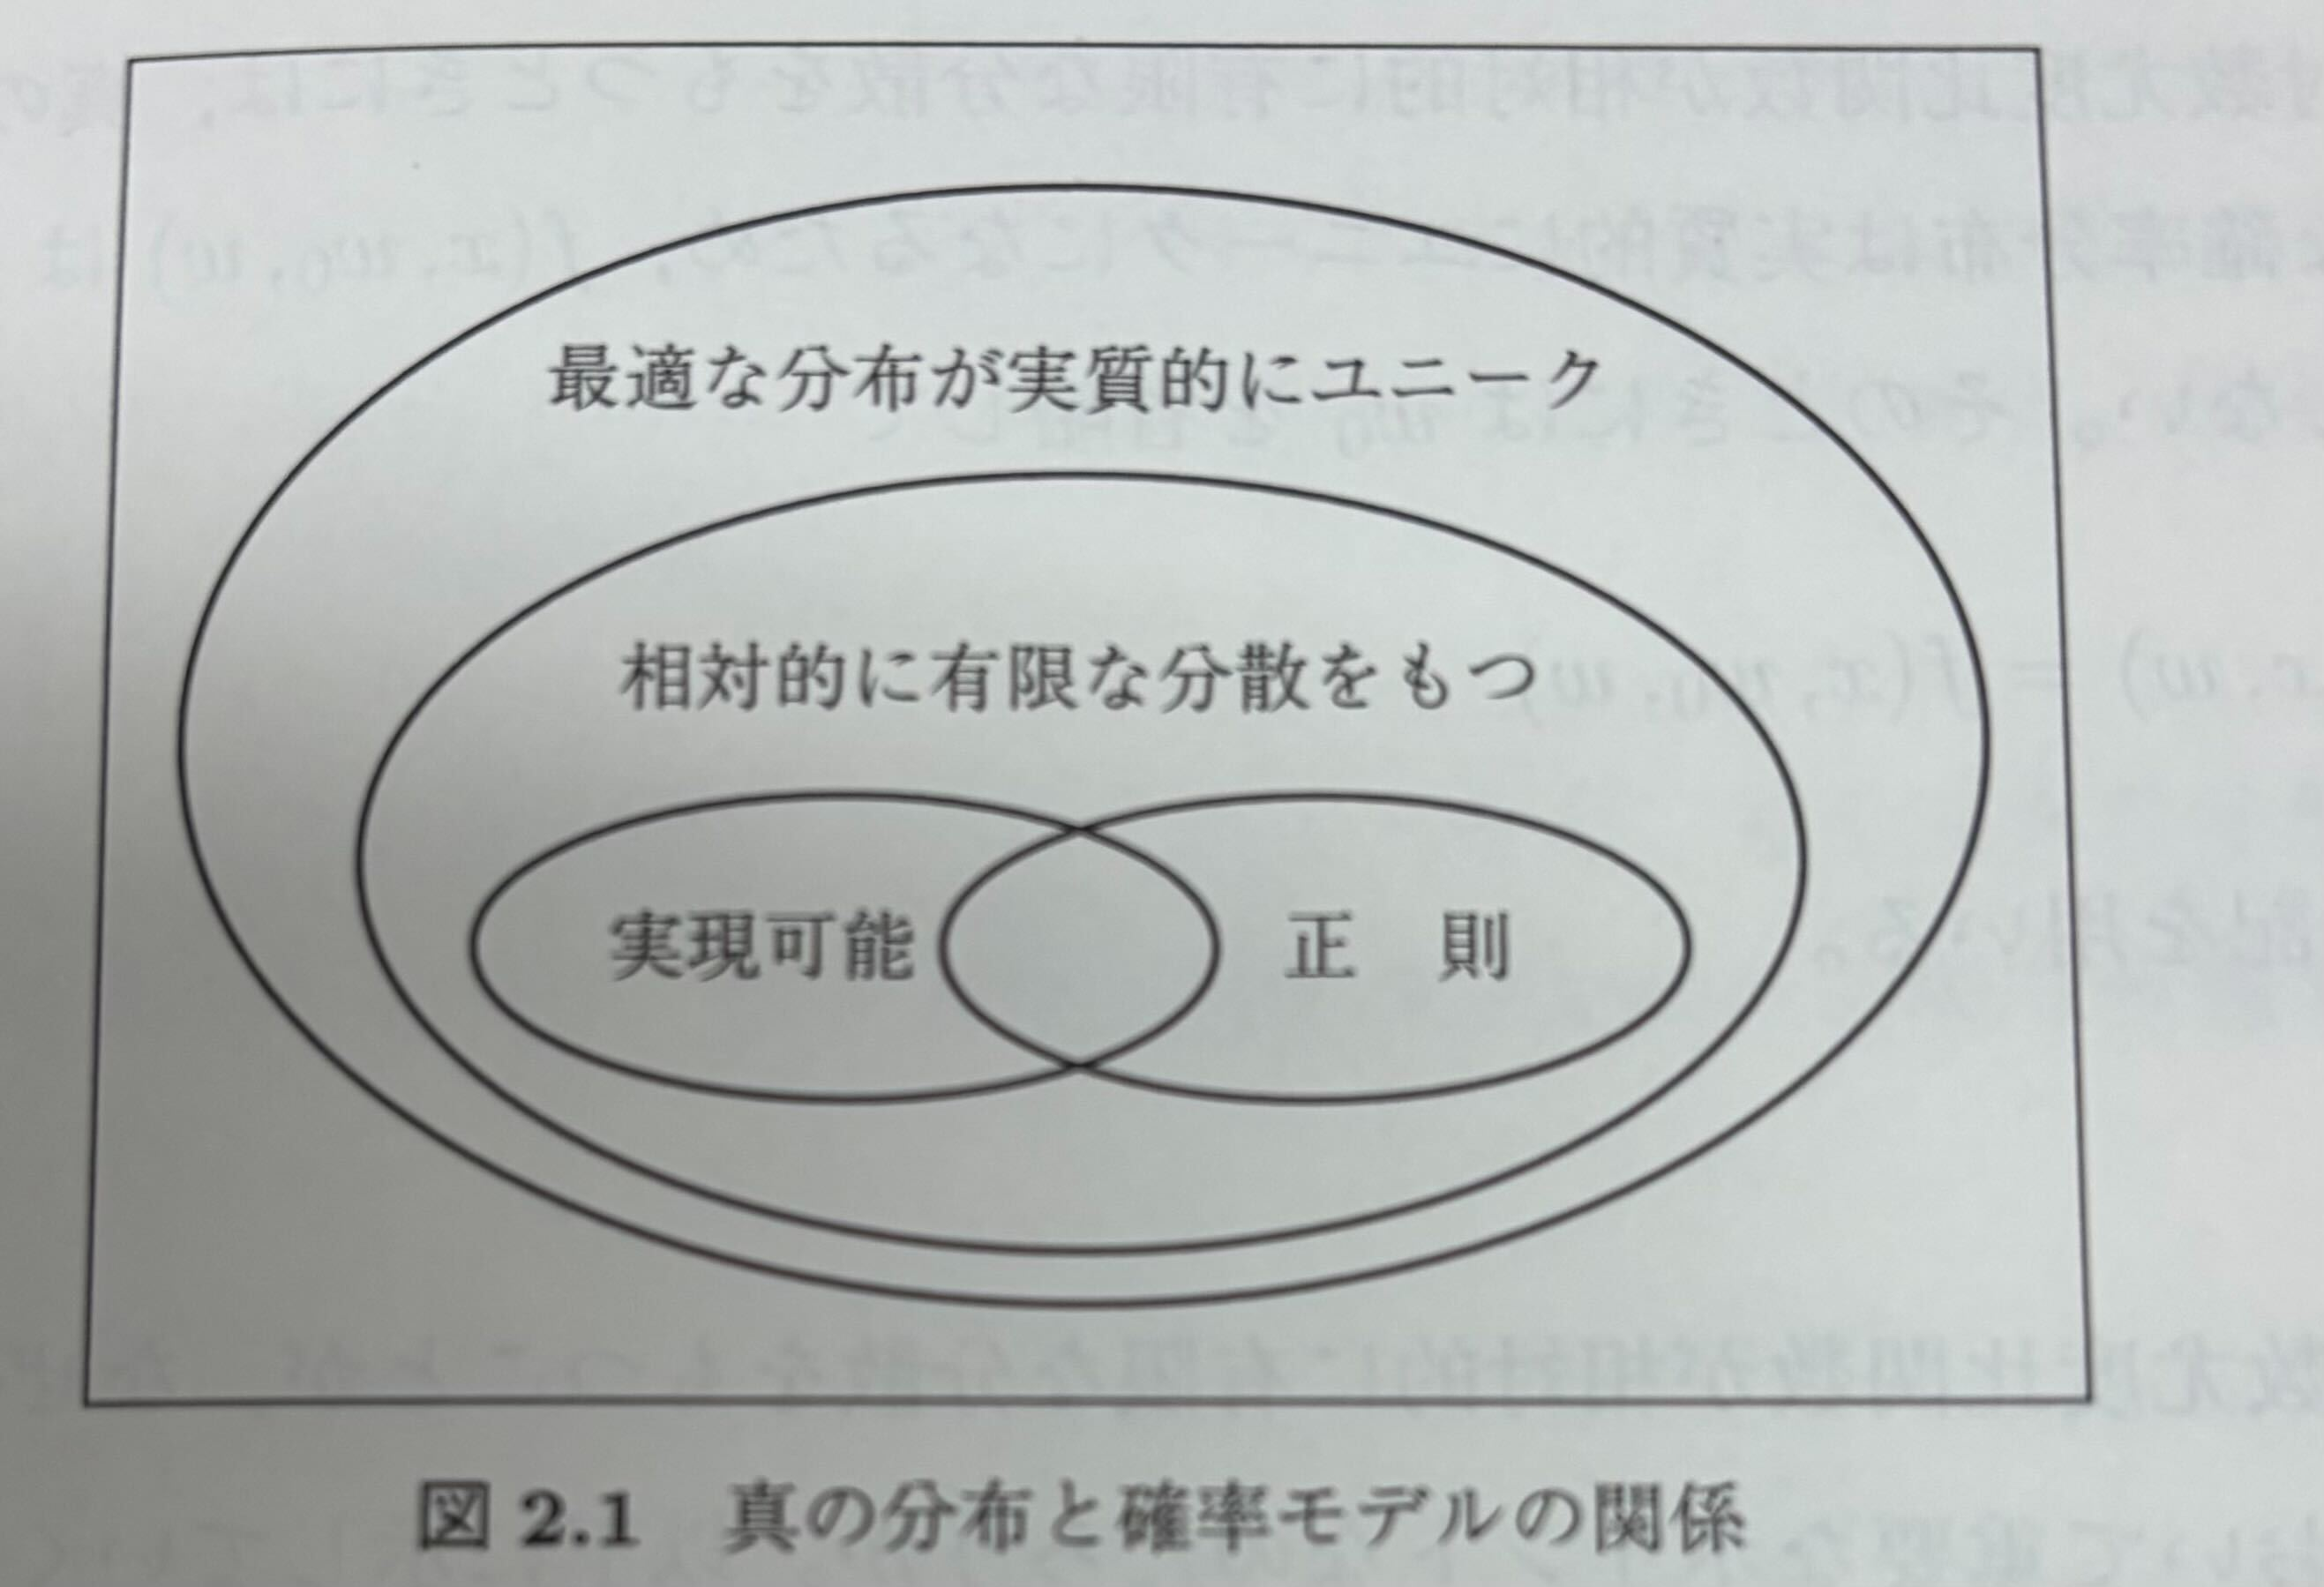
\includegraphics[width=0.5\textwidth]{yuugennnabunsan.jpg}
    \caption{真の分布と確率モデルに対する関係(渡辺ベイズ p35)}
    \label{fig:katei}
\end{figure}
以下の説明は、「相対的に有限な分散を持つ」ことが達成されている、すなわち「最適な分布が実質的にユニーク」な状況を前提にしている。
\newpage


\subsection{事後分布の期待値計算を行いたい}
本当は、任意のモデルと事前分布の設計に対して
\begin{equation}
    \ln\ev{p(X|w)}_{w|X^n}
\end{equation}
の計算を行いたい。しかしそれすら難しいので、$n$に対するオーダー評価で我慢する
\footnote{
    オーダー評価をしようと思うと、原理的に計算できない量$K(w)$を出現させる必要がある。これは収束先からのズレを見たいためしょうがないのか?
}。
$p(X|w)$は$n$に依存しない関数なので、事後分布が$n$に対してどのような振る舞いをしているかを見ればオーダー評価の意味では十分。
すなわち示すべきことは、$O(x,w)$を$n$に依存しない関数として、
\begin{equation}
    \ev{O(x,w)}_{w|X^n} \coloneqq \int O(x,w)p(w|X^n)\,\dd{w}\;。
\end{equation}
のオーダー評価を行うことである。それを実行するため、$p(w|X^n)$を天下り的だが(ラプラス近似を用いたいため)次のように変形する:
\begin{equation}
    p(w|X^n)\propto\varphi(w)\prod_{i=1}^{n}p(X_i|w)^{\beta} \propto \varphi(w)\exp(-n\beta K_n(w))\;。
\end{equation}
ここで$K_n(w)$は経験誤差関数であり、
\begin{equation}
    K_n(w) \coloneqq \frac{1}{n}\sum_{i=1}^{n}f(X_i,w) \coloneqq \frac{1}{n}\sum_{i=1}^{n} \ln{\frac{p(X_i|w_0)}{p(X_i|w)}}
\end{equation}
と定義される。なお、$f(x,w)$は対数尤度比関数と呼ばれ、$K_n(w)$は$f(x,w)$のサンプル平均である。
この変形を用いると、
\begin{equation}
    \ev{O(x,w)}_{w|X^n} = \frac{\int_{W} O(x,w)\exp(-n\beta K_n(w))\varphi(w)\,\dd{w}}{\int_{W} \exp(-n\beta K_n(w))\varphi(w)\,\dd{w}}
    \label{eq:expectation}
\end{equation}
となる。このように変形することで、事後分布の確率的な振る舞いを$K_n(w)$に押し付けることができた。
さらに指数関数の肩が$-n$に比例しているため、$n$が十分に大きな場合、
式\eqref{eq:expectation}の積分計算に寄与する領域は$K_n(w)$の最小値付近のみと考えることができる。
したがって、
\begin{enumerate}
    \item $K_n(w)$の最小値を取る点が、パラメータ空間$W$全体でどのような分布をしているか
    \item $K_n(w)$の最小値周りにおける関数の局所的な振る舞い
\end{enumerate}
を調べることが重要である。
$K_n(w)$の$w$に対する振る舞い方は、真の分布とモデル設計に依存して決まるため、第三章では正則理論という枠組みの元で$K_n(w)$の振る舞いを考える。
なお、$n\to\infty$極限における$K_n(w)$の収束先を平均誤差関数$K(w)$と呼ぶ:
\begin{equation}
    K_n(w)\to K(w) \coloneqq \mathbb{E}_{X}[f(X,w)] = \int f(x,w)q(x)\,\dd{x}\;。
\end{equation}
$K(w)$は真の分布$q(x)$とモデル設計方法$p(x|w)$に依存して決まる関数である。
\newpage


\subsection{期待値計算の評価において一般的に成り立つ事実}

\begin{mybox}[期待値計算における積分の分割]
    事後分布による期待値計算は以下の形で表される:
    \begin{equation}
      \ev{O(x,w)}_{w|X^n}=\frac{\int_{W} O(x,w)\exp(-n\beta K_n(w))\varphi(w)\,\dd{w}}{\int_{W} \exp(-n\beta K_n(w))\varphi(w)\,\dd{w}}\;。
    \end{equation}
    分母は分子の積分において$O(x,w)=1$を代入した形であるため、分子の$n$に対する振る舞いを見れば全体の振る舞いがわかる。
    分子の積分領域を2つに分割し、$n$に対する主要項(第一項目)、非主要項(第二項目)へと分割する:
    \footnote{
        主要項、非主要項という言葉は、各項のオーダー評価が意味をなすくらい$n$が大きな領域ということを前提に使っている。
        また、二項目が非主要項であることは、第一項目の評価を行って初めて分かる事実ではあるが、それは認めてください。
    }
    \footnote{
        $O(x,w)$は$n$に依存していない関数であることを前提としており、これが$n$に依存していればオーダー評価も変わってくる。
    }
    \begin{equation}
         \int_{K(w)<\epsilon_n} O(x,w)\exp(-n\beta K_n(w))\varphi(w)\,\dd{w} + \int_{K(w)\geq \epsilon_n} O(x,w)\exp(-n\beta K_n(w))\varphi(w)\,\dd{w}\;。
    \end{equation}
    ただし、値$\epsilon_n>0$は$n$の単調減少関数であり、
    \begin{equation}
        \lim_{n\to\infty} \epsilon_n = 0 ,\quad \lim_{n\to\infty} \sqrt{n}\epsilon_n = \infty
    \end{equation}
    を満たすように選ぶ。このとき、非主要項(第二項目)は正則理論の仮定なしで、
    \begin{equation}
        \int_{K(w)\geq \epsilon_n} O(x,w)\exp(-n\beta K_n(w))\varphi(w)\,\dd{w} = o_p(\exp(-\sqrt{n}))
    \end{equation}
    になることが示される。この事実を示すために必要なのは$K_n(w)$の$n$に対する振る舞いの調査のみであり、正則理論の仮定は必要なく常に成り立つ。したがって、
    \begin{equation}
        \ev{O(x,w)}_{w|X^n} = \frac{\int_{K(w)<\epsilon_n} O(x,w)\exp(-n\beta K_n(w))\varphi(w)\,\dd{w}}{\int_{K(w)<\epsilon_n} \exp(-n\beta K_n(w))\varphi(w)\,\dd{w}} + o_p(\exp(-\sqrt{n}))\;。
    \end{equation}
    が常に成立する。なお、$K(w)$がでてきているので、計算できない量になっているのは注意。
\end{mybox}
以降は主要項
\begin{equation}
    \int_{K(w)<\epsilon_n} O(x,w)\exp(-n\beta K_n(w))\varphi(w)\,\dd{w} 
\end{equation}
のオーダー評価を行う。$K(w)$に性質の良い仮定を課してオーダー評価を行っているのが正則理論(第三章)であり、そうでない場合は一般理論(第四章)である。
\footnote{
    $K_n(w)$ではなく$K(w)$に仮定を課していることには注意。正則理論の枠組みでは、$K(w) < \epsilon_n$の領域内部において
    \begin{equation}
        \exp(-n\beta K_n(w))\propto  \mathcal{N}\qty(w_0 + \hat{\xi}_n/\sqrt{n}, (n\beta J(w_0))^{-1})(1+o_p(1))
    \end{equation}
    と表される。なお、$J(w_0)$は正定値行列で、$J(w)=\laplacian{K(w)}$と定義されている。また、$\hat{\xi}_n$は$K_n(w_0)$の確率的な振る舞いを担う確率変数である。
    積分領域はこの分布の広がりよりも十分に大きく、$\mathbb{R}^d$全体での積分に置き換えてGauss積分が適用できる。
}

\section{正則理論}
\subsection{正則理論での仮定}
正則理論とは、真の分布とモデル設計(と、サンプルの数)が、以下の3つの条件を満たすことを仮定する理論である
\footnote{
    渡辺ベイズ本では$K(w)$ではなく$L(w)$についての仮定をしていたが、これらは基準点を変えただけであり、
    \begin{equation}
        L(w) = L(w_0) + K(w)
    \end{equation}
    によって結びつけられるため、$K(w)$に関する仮定として考えても良い。なお、$L(w)$は平均対数損失であり、
    \begin{equation}
        L(w) = -\mathbb{E}_X[\ln{p(X|w)}]
    \end{equation}
    と定義される。
}:
\begin{enumerate}
    \item $K(w)$を最小にするパラメータが唯一$w_0$である。これは、最適なパラメータの集合が$W_0=\{w_0\}$と表されることと同じ意味である。
    \item $K(w)$のHessian:$J(w)=\laplacian{K(w)}$に対し、$J\coloneqq J(w_0)$が正定値である。
    \item サンプルの数$n$が十分に大きいこと。
\end{enumerate}

これらの仮定によって、
\begin{itemize}
    \item 主要項の積分範囲を考える際には$w=w_0$の近傍のみでよくなる。
    \item $w=w_0$近傍で主要項の被積分関数はGaussianとして扱える。
\end{itemize}
という嬉しい性質が成り立つ。結論だけ述べると、この仮定の元で主要項のオーダー評価は次のようになる。
\begin{mybox}[期待値のオーダー評価(正則理論の場合)]
    正則理論という仮定を課している場合、以下のオーダー評価が成立する:
    \begin{align}
    \ev{O(x,w)}_{w|X^n} = \frac{\int_{\mathbb{R}_d} O(x,w)\exp(-\frac{n\beta}{2}\norm{J^{1/2}\qty(w-w_0-\frac{\hat{\xi}_n}{\sqrt{n}})}^2)\dd{w}}
    {\int_{\mathbb{R}_d} \exp(-\frac{n\beta}{2}\norm{J^{1/2}\qty(w-w_0-\frac{\hat{\xi}_n}{\sqrt{n}})}^2)\dd{w}}(1+o_p(1))\;。
    \end{align}
\end{mybox}
2章の残りでは、この計算途中で大事だと思われる式変形について説明する。
\newpage

\subsection{正則理論で用いる文字の定義}
正則理論の仮定の元での主要項の振る舞いの結果を述べる前に、少しだけ文字の定義を行う。
まずは$K_n(w)$を次のように変形する:
\begin{equation}
    K_n(w) = K(w) - (K(w)-K_n(w)) = K(w) - \frac{1}{\sqrt{n}}\eta_n(w)\;。
\end{equation}
ここで$\eta_n(w)$は$K_n(w)$の確率的な振る舞い方を担う確率過程であり、次のように定義される:
\begin{equation}
    \eta_n(w)\coloneqq \frac{1}{\sqrt{n}}\sum_{i=1}^{n}(K(w)-f(X_i,w))\;。
\end{equation}
この確率過程は経験過程と呼ばれるものであり、$n\to\infty$でとある確率過程に法則収束するという良い性質を持っている。
この性質があることで、収束先の確率分布からのズレとして$K_n(w)$をオーダー評価することが可能になる。必要となる確率変数$\xi_n,\,\hat{\xi}_n$を
\begin{align}
    \xi_n &= J^{-1/2}(w_0)\grad{\eta_n(w_0)} \;、\\
    \hat{\xi}_n &= J^{-1/2}(w_0)\xi_n = J^{-1}\grad{\eta_n(w_0)}
\end{align}
と定義する。$\grad{\eta_n(w)}$がすべての$w$で$\mathcal{N}(0,I(w))$に法則収束するという性質を持っているため、
\begin{itemize}
    \item 確率変数$\xi_n$は正規分布$\mathcal{N}(0,J^{-1/2}IJ^{-1/2})$に法則収束する。
    \item 確率変数$\hat{\xi}_n$は正規分布$\mathcal{N}(0,J^{-1}IJ^{-1})$に法則収束する。
\end{itemize}
ここで$I=I(w_0)$であり、$I(w)$は以下で定義される:
\begin{equation}
    I(w) \coloneqq \mathbb{E}_{X}\qty[\grad{f(X,w)}(\grad{f(X,w)})^\top] - \grad{K(w)}(\grad{K(w)})^{\top}\;。
\end{equation}

\subsection{正則理論における主要項のオーダー評価}
正則理論の仮定のもとでは、$w=w_0$近傍の$K_n(w)$の振る舞いを見れば良い。
$K_n(w)$を平方完成してGauss積分として扱いたいため、平均値の定理を利用して$w=w_0$周りの展開を考える。
そのため
\begin{equation}
    K_n(w) = K(w) - \frac{1}{\sqrt{n}}\eta_n(w)
\end{equation}
の右辺の項にそれぞれ平均値の定理を用いると、$w$により定まる2つの値$w^*,\,w^{**}$が存在し、
\begin{align}
    K(w) &= \frac{1}{2}(w-w_0)\cdot J(w^*)(w-w_0)\;, \\
    \eta_n(w) &= (w-w_0)\cdot \grad\eta_n(w^{**})\;。
\end{align}
が成立する。$K(w)$の一次項が出てこないのは、$\grad K(w_0)=0$が成立しているためである。
これらの結果から、$K_n(w)$は$w$の二次式として表される:
\begin{equation}
    K_n(w) = \frac{1}{2}(w-w_0)\cdot J(w^*)(w-w_0) - \frac{1}{\sqrt{n}}(w-w_0)\cdot\grad\eta_n(w^{**})\;。
\end{equation}
なお、平方完成を行うためには$J(w^*)$が正則(対角化可能)であることが必要である。
渡辺ベイズ本では、$w^*$が$w_0$近傍では$J(w^*)$が常に正則ということを仮定しているが、その妥当性がどこから来ているのかは不明。
正則であることを認めたうえで、$K_n(w)$は
\begin{equation}
    nK_n(w) = \frac{n}{2}\norm{J(w^*)^{1/2}\qty(w-w_0-\frac{1}{\sqrt{n}}J(w^*)^{-1}\grad\eta_n(w^{**}))}^2 
    - \frac{1}{2}\norm{J(w^*)^{-1/2}\grad\eta_n(w^{**})}^2
\end{equation}
と平方完成できる。

また、$n\to\infty$のとき$\epsilon_n\to 0$であり、正則理論の仮定1のおかげで、$w^*,\,w^{**}\to w_0$が成立する。したがって一般の$n$ではそこからのズレとして
\begin{equation}
    J(w^*) = J + o_p(1) ,\quad \grad\eta_n(w^{**}) = \grad\eta_n(w_0) + o_p(1)
\end{equation}
が成立する。このオーダー評価の結果を用いると、主要項は次のように表せる:
\begin{align}
    &\int_{K(w)<\epsilon_n} O(x,w)\exp(-n\beta K_n(w))\varphi(w)\,\dd{w} \notag \\
    =& \exp(\frac{\beta}{2}\norm{\xi_n}^2)\varphi(w_0)\int_{K(w)<\epsilon_n} O(x,w)\exp(-\frac{n\beta}{2}\norm{J^{1/2}\qty(w-w_0-\frac{\hat{\xi}_n}{\sqrt{n}})}^2)\dd{w}(1+o_p(1)) \notag \\
    =& \exp(\frac{\beta}{2}\norm{\xi_n}^2)\varphi(w_0)\int_{\mathbb{R}^d} O(x,w)\exp(-\frac{n\beta}{2}\norm{J^{1/2}\qty(w-w_0-\frac{\hat{\xi}_n}{\sqrt{n}})}^2)\dd{w}(1+o_p(1))\;。
\end{align}
最後の等式は、積分範囲を$\mathbb{R}^d$全体に広げてもよいということを利用している。これにより、先ほど提示したオーダー評価の形が得られる:
\begin{mybox}[期待値のオーダー評価(正則理論の場合)]
    正則理論という仮定を課している場合、以下のオーダー評価が成立する:
    \begin{align}
    \ev{O(x,w)}_{w|X^n} = \frac{\int_{\mathbb{R}_d} O(x,w)\exp(-\frac{n\beta}{2}\norm{J^{1/2}\qty(w-w_0-\frac{\hat{\xi}_n}{\sqrt{n}})}^2)\dd{w}}
    {\int_{\mathbb{R}_d} \exp(-\frac{n\beta}{2}\norm{J^{1/2}\qty(w-w_0-\frac{\hat{\xi}_n}{\sqrt{n}})}^2)\dd{w}}(1+o_p(1))\;。
    \end{align}
\end{mybox}

\newpage
\section{正則理論における汎化損失の振る舞い}
正則理論においては、事後分布による期待値計算のオーダー評価が可能になった。その結果を用いると$G_n$は
\begin{equation}
    G_n = -\mathbb{E}_X\qty[\ln\ev{p(X|w)}_{w|X^n}] = L(w_0) + \frac{1}{n}\qty(\frac{d}{2\beta} + \frac{1}{2}\norm{\xi_n}^2 - \frac{1}{2\beta}\tr{IJ^{-1}}) + o_p\qty(\frac{1}{n})
\end{equation}
となる。これには原理的に計算が不可能な量が入っており、これは
\begin{itemize}
    \item 真の分布による期待値を外から取ったから
    \item 事後分布の期待値計算をオーダー評価するために収束先の値を見たから
\end{itemize}
という2つの理由がある。真の分布をしらないと計算不可能な量は
\begin{align}
    L(w_0) &= -\mathbb{E}_X[\ln{p(X|w_0)}]\;,  \\
    \xi_n &= J^{-1/2}\grad{\eta_n(w_0)}\;, \\
    I = I(w_0) &= \mathbb{E}_{X}\qty[\grad{f(X,w_0)}(\grad{f(X,w_0)})^\top] - \grad{K(w_0)}(\grad{K(w_0)})^{\top}\;, \\
    J = J(w_0) &= \laplacian{K(w_0)}
\end{align}
である。また、$w_0$の値も真の分布をしらないと求められない。いったいこれからどうするのか。ちなみに経験損失$T_n$は原理的に計算できる:
\begin{equation}
    T_n = -\frac{1}{n}\sum_{i=1}^{n}\ln\ev{p(X_i|w)}_{w|X^n}\;。
\end{equation}
経験損失のオーダー評価は
\begin{equation}
    T_n = L_n(w_0) + \frac{1}{n}\qty(\frac{d}{2\beta}-\frac{1}{2}\norm{\xi_n}^2-\frac{1}{2\beta}\tr{IJ^{-1}}) + o_p\qty(\frac{1}{n})
\end{equation}
となる。
\begin{align}
    L_n(w_0) = -\frac{1}{n}\sum_{i=1}^{n}\ln{p(X_i|w_0)}\;, \\
\end{align}
は$\omega_0$を別の量に置き換えれば計算可能ではある。
また、サンプルによる期待値を取ると、
\begin{align}
    \mathbb{E}[G_n] &= L(w_0) + \frac{1}{n}\qty(\frac{\lambda-\nu}{\beta}+\nu) + o\qty(\frac{1}{n})\;, \\
    \mathbb{E}[T_n] &= L(w_0) + \frac{1}{n}\qty(\frac{\lambda-\nu}{\beta}-\nu) + o\qty(\frac{1}{n})
\end{align}
と表される。ここで
\begin{equation}
    \lambda=\frac{d}{2},\quad \nu=\frac{1}{2}\tr{IJ^{-1}}
\end{equation}
である。

\newpage

\section{Bayes推測以外の方法で予測分布を構成する}
予測分布の構成方法としてBayes推測以外の手法を用いた場合にどのようになるかを説明する。
特に、最尤推定法と事後確率最大化法(MAP推定法)が統一的に説明できることを述べる。これらはパラメータを点推定するような方法である。
まず、ハイパーパラメータ$\beta>0$に依存する関数
\begin{equation}
    \mathcal{L}_n(\beta) \coloneqq -\frac{1}{n}\sum_{i=1}^{n}\ln{p(X_i|w)} - \frac{1}{n\beta}\ln{\varphi(w)}
\end{equation}
を最小にするパラメータを$\hat{w}^{\beta}_{n}$とおく。このようなパラメータが唯一とは限らない。
このとき、予測分布を
\begin{equation}
    p_n^{*}(x) = p(X|\hat{w}^{\beta}_{n})
\end{equation}
と定義する。$\beta\to\infty$とした場合が最尤推定
\footnote{
    最尤推定はデータを完全に信じてモデルの対数尤度を最大化するパラメータを選択するような推定方法であるため過学習を起こしやすい?
}
であり、$\beta=1$とした場合が事後確率最大化法(MAP推定)に対応する。
すなわち$\beta$は事前分布と学習データをどれくらい重視するかを調整する意味を持っている。


\begin{mybox}[推定量の一致性]
    式\eqref{eq:optimal-parameter-set}で定義した集合$W_0$の元が唯一$w_0$であるとき、
    任意の$\beta$について、$n\to\infty$のとき$K(\hat{w}_n^{\beta})$の値は$0$に確率収束する。
    また、正則理論を仮定していれば、$\hat{w}_n^{\beta}\to w_0$に確率収束する。
\end{mybox}





\newpage

\section{情報量規準}
この章は自分の中でその意味を捉えられていないまま書いています。
\begin{itemize}
    \item $G_n$そのものを情報量規準で推定したいわけではない?
    \item $G_n$のオーダー評価の結果を用いて計算できない量は微小量として扱えるようにし、主要項は計算できる量で推定したい?
    \item $\mathbb{E}[G_n]$の意味で、主要項は計算できる量で推定したい?
\end{itemize}

\subsection{BIC}
BICの定義は次である:
\begin{equation}
    \text{BIC} \coloneqq -\sum_{i=1}^{n}\ln{p(X_i|\hat{w}_n^{\beta})} + \frac{d}{2}\ln{n}
\end{equation}

複数のモデルの比較においてBICが小さいほど適切であると考えるとき、この値のことをベイズ情報量規準という。

BICは、真の分布は単純なモデルで表現できるということがわかっているときに使うような指標だと思った。
BICが他の指標と違うのは、$n$に比例する項が入っていることであり、たとえば$n\to\infty$を考える(真の分布が再現できるほどデータが与えられている)場合を考えると、
任意の$X\sim q(x)$に対して$p(X|\hat{w})$がゼロにならない$\hat{w}$が存在するくらいの表現能力を持つ$d$の中で、一番小さい$d$をもつモデルを選ぶことになる。
つまり真の分布を再現できる表現能力を持つもののうち、最も単純なモデルが選ばれる

\begin{mybox}[BICについて定性的に理解する]
    解釈をしやすくするために$d$が同じモデルを2つ持ってきて、$\beta$も固定する。データセットも同じものを用意する。事前分布も同じにする。
    もっともらしいパラメータ$\hat{w}_{n}^{\beta}$を決めたとき、BICが小さいほうが適切ということは、予測分布$p_n^{*}(x)$に関する対数尤度
    \begin{equation}
        \sum_{i=1}^{n}\ln p_n^{*}(X_i)
    \end{equation}
    が大きいモデルのほうが適切であるということを意味する。これは最尤推定法を擬似的に利用したいということ?
    また、表現能力が必要以上に高すぎると過学習のおそれがあるので、同じくらいの表現能力を持っているモデルでは、よりパラメータが少ないモデルを選択している。
    これ以上の意味はわからない。自由エネルギーの主要項がBICそのものらしいので、自由エネルギーの意味を理解しないといけない気がする。
\end{mybox}


\newpage
\subsection{RIC}
RICの定義は次である:
\begin{equation}
    \text{RIC} \coloneqq T_n + \frac{1}{n}\tr{IJ^{-1}}\;。
\end{equation}
これは計算できない量である。しかし、RICの$1/n$よりも大きなオーダー項はすべて計算できる量としてまとめられる:
\begin{equation}
    \text{RIC} = L_n(\hat{w}_n^{\beta}) + \frac{1}{n}\qty(\frac{d}{2\beta} + \qty(1-\frac{1}{2\beta}\tr{I_n(\hat{w}_n^{\beta})J_n(\hat{w}_n^{\beta})^{-1}})) + o_p\qty(\frac{1}{n})\;。
\end{equation}
ここで計算できる新たな量として
\begin{align}
    I_n(w) &\coloneqq \frac{1}{n}\sum_{i=1}^{n}\grad{\ln{p(X_i|w)}}(\grad{\ln{p(X_i|w)}})^{\top} \\
    J_n(w) &\coloneqq -\frac{1}{n}\sum_{i=1}^{n}\laplacian\ln{p(X_i|w)} \\
\end{align}
を定義した。この量は、大数の法則と$\hat{w}_n^{\beta}\to w_0$を用いて
\begin{equation}
    I(w_0)=I_n(\hat{w}_n^{\beta}) + o_p(1),\quad J(w_0) = J_n(\hat{w}_n^{\beta}) + o_p(1)
\end{equation}
となることが示せるらしい。

RICでは常に
\begin{equation}
    \mathbb{E}[G_n] = \mathbb{E}[\text{RIC}] + o\qty(\frac{1}{n})
\end{equation}
が成立する。よって$1/n$より大きなオーダーにおいて、汎化損失$G_n$のサンプル期待値を推定したいのが目的な気がする。
本当はチューニングしきったモデルの中で$G_n$が小さくなる方がどちらであるかを見たいんだけど、それが難しくてサンプル期待値の意味でしか見れないということ。

\subsection{TIC}
TICはいらない。RICと完全に同じ意味を持つと思う。Bayes以外の推定方法に対応する汎化損失を使ってるだけ。

\subsection{AIC}
AICは大事な量である。実現可能な場合の話をしていたのは、単純に平均が一致することを示したかったためだけだと思う。たしかに実現可能だったらAICはRICと同じになる。

AICは感度が高い(サンプルに依存して判定が変わってしまう)ような指標である。

このような指標で選ばれ続けるモデルは、どのようなサンプルが与えられても適切なモデル(AICの意味で常に低い量を出し続けるモデル)と解釈できる。
つまり新しいサンプルに対して堅牢なモデルを選びたいときに使う気がする。AICとBICの用途は完全に違うものな気がする。


BICは感度が低い。つまりサンプルが信頼できるような場合に使えるもの。信頼できないのに感度が低い指標を使っちゃうと、決めつけで適当なモデルになる。



\end{document}
